\documentclass[10pt]{article}
\usepackage[margin=1in]{geometry}
\usepackage[utf8]{inputenc}
\usepackage{mathtools}
\usepackage{amsthm, amssymb}
\usepackage{subcaption}

\def\bbone{\text{\usefont{U}{bbold}{m}{n}1}}
\def{\Ex}{\mathbb{E}}% expected value

\newcommand{\gp}{\mathcal{GP}}
\newcommand{\Normal}[2]{\mathcal{N}\left( #1 , #2 \right)}



\usepackage[T1]{fontenc}
\usepackage{graphicx}


\usepackage{tikz}
\usetikzlibrary{fit,positioning,calc,shapes,backgrounds}
\usetikzlibrary{shapes.geometric, arrows}

\theoremstyle{definition}
\newtheorem{definition}{Definition}[section]

\author{Charlie}
\title{Background Estimation and Fit Studies}
\date{2024-02-23}
\begin{document}
\section{Gaussian Process Regression}

Gaussian process regression is a statistical learning technique that permits a computationally tractable description of a "distribution of functions."
Specifically, a gaussian process is a non-parametric model that allows do regression without explicitly specifying a form that the fit should take.
This makes it especially useful for QCD background estimation, where there is no apriori description for the background, often resigning analyses to pick a random function that seems to fit the data. 

\subsection{Mathematical Description}

\begin{definition}
  A Gaussian Process (GP) is a stochastic process for which any finite subset of the random variables is jointly gaussian. 
\end{definition}


Being a gaussian, a GP $f(x)$ is defined by its mean and its covariance.
\begin{align}
  m(x) &= \Ex\left(f(x)\right) \\
  k(x,x') &= \Ex\left( ( f(x) - m(x) ) (f(x') - m(x'))\right) 
\end{align}
We write such a process as $\gp(m(x), k(x,x'))$. Note that in this case, the random variables are $f(x)$, meaning there is a separate random variable for each value of $x$.
In common statistics language, $x$ plays the role of the index in a random process.

Note that there is an inherent self-consistency requirement here. If we are looking at some collections of points $X_1$ and another collection $X_2$ then the process must behave consistently regardless of whether we look at the join distribution of $X_1 + X_2$ or the sets separately.

Since a multivariate gaussian has this property inherently, everything works out if $k(x,x') = C_{x,x'}$ where $C$ is the multivariate covariance. 

\subsection{Distribution}

The combination of the mean,covariance, and self-consistency requirements means that a Gaussian process described a distribution over a space of functions. Specifically, if we select test points $X_{*}$ then the
\begin{align}
  P(f_{*}) \sim \Normal{m(X_{*})}{k(X_{*},X_{*})}
\end{align}

\subsection{Training}

Ultimately we want to perform regression: taking known data and extrapolating in to some unknown region.
To accomplish this we need to be able adapt our GP based on some known observations.
This is precisely the domain of Baye's theorm: taking a prior distribution and some data, and forming a posterior distribution that describes our updated belief in the model.

Because the normal distribution behaves very nicely under conditioning and marginalization, we can actually do this process with direct appear to Baye's theorem.

In general, we have some noisy data $y = f(x) + \sigma$, where $\sigma$ gaussian distributed noise.
Then we can write
\begin{align}
  cov(y) = K(X,X) + I \sigma_n^{2}
\end{align}

Then the joint distribution of our noisy training points and our test points -- the points where we want to perform regression -- is
\begin{align}
  \label{}
  \begin{bmatrix}
    y \\
    f_{*}  
  \end{bmatrix}
  =
  \Normal{
  \begin{bmatrix}
    X \\
    X_{*}
  \end{bmatrix}
  }{
  \begin{bmatrix}
    K(X,X) + I \sigma_X^2 & K(X, X_{*}) \\
    K(X_{*},X)  & K(X_{*}, X_{*}) 
  \end{bmatrix}
  }
\end{align}

However, in almost all cases, the mean is set to 0, since 

Conditioning this Gaussian distribution on the observed values $y$ gives the posterior distribution over the test points $X_{*}$. 

\begin{align}
  m(X_{*})  &= \Ex \left[ f_{*} | X,y,X_{*}\right]  = K(X,X_{*}) \left( K(X,X) + \sigma_X^2 I \right)^{-1} y \\ 
  K(X_{*}, X_{*})  &= cov(f_{*}) = K(X_{*},X_{*}) - K(X_{*},X)\left( K(X,X) +\sigma_X^2 I \right)^{-1} K(X,X_{*})
\end{align}

This is most tractable represented by considering a single test point $x_{*}$:
\begin{align}
  \label{eq:single-point-pred}
  \Ex\left[f(x_{*})\right] &=  k(X, x_{*})^{T} \left( K(X,X)  + \sigma_X^2 I \right)^{-1} y \\
  Var(x_{*})  &=  K(x_{*},x_{*}) - K(x_{*},X)^{T}\left( K(X,X) +\sigma_X^2 I \right)^{-1} K(X,x_{*})
\end{align}

The mean prediction for the point $x_{*}$ is a linear combination of the test points $y$ weighted by their covariance with the test point. The variance of the point is simply the prior variance, modified some term involving only the training points (not their values). 

\subsection{Kernel Rundown}

In most problems, the mean is simply taken to be zero, since it can always be added back, and in most cases the posterior mean adapts very well.

Of much greater interest is the kernel function. This is really the function that determines the behavior of the process, and is the subject of most study.
This is perhaps not surprising -- it is the kernel that determines how different datapoints interact, and so it is ultimately the kernel that furnishes predictive power.

Below we provide a rundown of some covariance functions.

\subsubsection{RBF}
The archetype for kernels is the Radial Basis Function, sometimes called the squared-exponential kernel. It is defined as
\begin{equation}
  \label{}
  k(x,x') = e^{-\frac{(x-x')^{2}}{\ell^{2}}}
\end{equation}
In multiple dimensions, such a kernel could instead be 
\begin{equation}
  k(x,x') = e^{-(x-x')^{T} M (x-x')}
\end{equation}
where M is positive semidefinite, to ensure that this is, in fact, a kernel.
This is the most frequently used kernel for GPs.

\subsubsection{Matern Kernels}

A generalization of the RBF kernel is the Matern kernel
\begin{equation}
  k(x,x') = \frac{2^{1-\nu}}{\Gamma{\nu}} \left( \frac{(x-x')\sqrt{2\nu}}{\ell} \right)^{\nu} K_{\nu}\left(  \frac{(x-x')\sqrt{2\nu}}{\ell} \right)
\end{equation}

\subsubsection{Rational Quadratic Kernel}
The rational quadratic kernel is an infinite sum of RBF kernels with different length scales
\begin{equation}
  k(x,x') = \left( 1 + \frac{ \left( x -x' \right)^2 }{2 \alpha \ell^2} \right)^{-\alpha}
\end{equation}

\subsection{Model Selection}
Thus far, all our prediction have assumed an existing form for our kernel, both in type and in choice of hyperparameters.
In the real world, however, we need a method of determining these things obervationally.

The general conclusion is: select the model that minimizes the log marginal likelihood. 

\section{Regression for Combinatorial Backgrounds}
\label{sec:regression-for-qcd}

In this ever growing section, we present ongoing work on developing background estimation in both 1 and 2 dimension space for combinatorial backgrounds.

The gist of the procedure for estimating the background for a certain mass point is this:
\begin{itemize}
\item Blind a window of size and shape X around the mass points
\item Using a kernel X optimize the hyperparameters using this exterior region
\item Use GP regression to estimate the background within the signal area. 
\end{itemize}
Fundamentally, what is needed is a choice of window blinding area and kernel that allows for an accurate estimation of the background within the blinded in region.
In two dimensions, this problem is much more challenging, since there is additional structure in 2 dimensions that disobeys the normal ``smoothly falling everywhere'' the prevails in 1 dimension. 

\textbf{We want to develop a gaussian process procedure that can accurately estimate the background in a blinded window of various sizes.}

\subsection{Points of Interest}

There is a substantial amount of ``parameter'' space to cover as we work towards the determination of a good procedure.
We want to study how the below interact in isolation and with each other.
\begin{description}
\item[Kernel] The choice of kernel is the most important aspect of the GP. 
\item[Window Size/Shape] The size and shape of the blinding window. 
\item[Valid Region] The region of space we examine the regression, in particular if we exclude zero event bins.
\item[Mean] The choice of mean function.
\item[Binning] How bin size influences the fit.
\end{description}

We want to not only accurately estimate the background in the blinded region, but also be robust against variations in shape, binning, statistics, etc.


The majority of our efforts currently revolve around trying to determine an optimal kernel for the regression.


\section{Kernel Studies}
\label{sec:kernel-studies}

The choice of kernel is the most important aspect of Gaussian process regression.
Here we document efforts to determine a kernel that provides both a flexible and accurate estimation of the background in the signal window.

We first do studies on the complete plane. 
This is used to determine if the fit is flexibile enough to accurately capture the features of the background.


\newcommand{\makegrid}[3]{
  \begin{figure}[ht]
    \centering
    \begin{subfigure}[b]{0.45\textwidth}
      \centering
      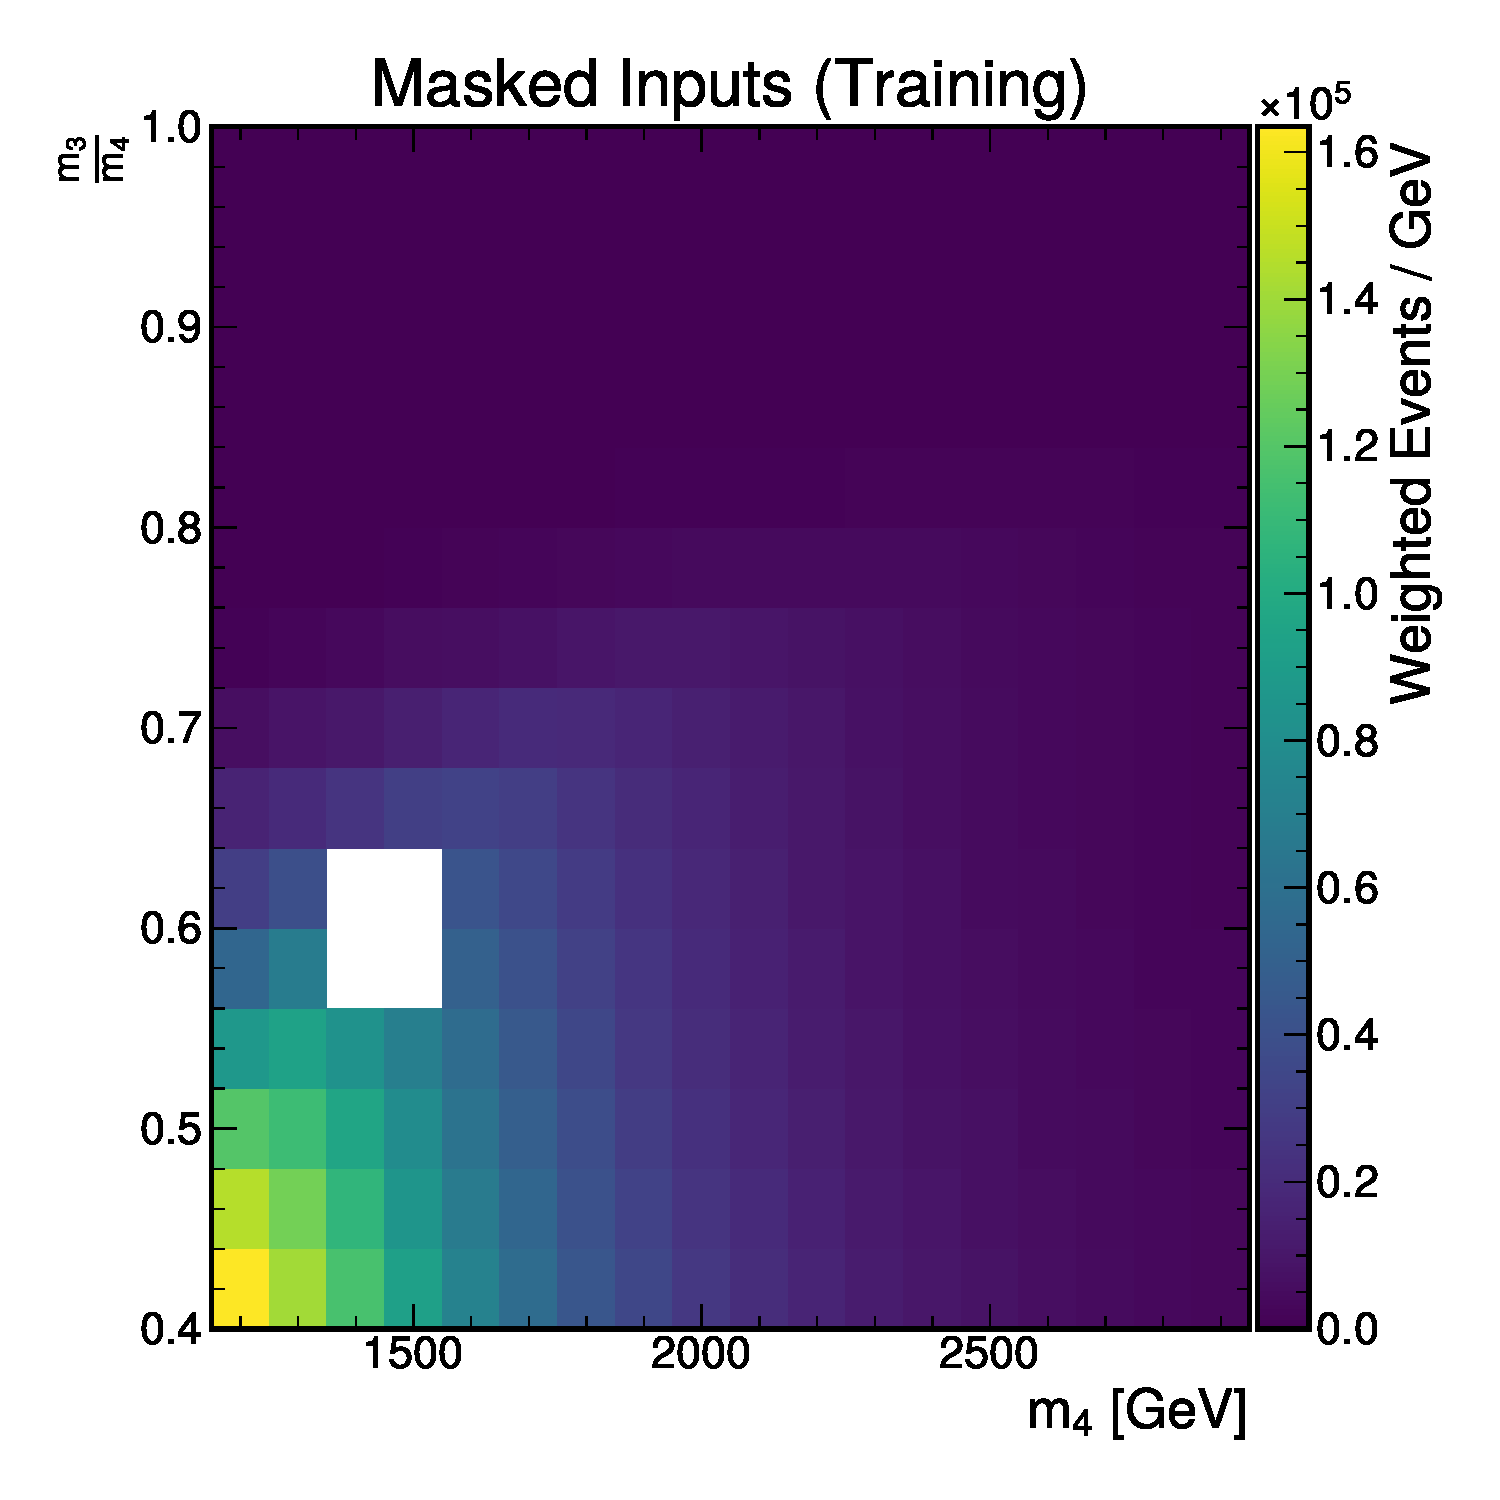
\includegraphics[width=\linewidth]{figures/#1/training_points.pdf}
      \caption{}
    \end{subfigure}
    \begin{subfigure}[b]{0.45\textwidth}
      \centering
      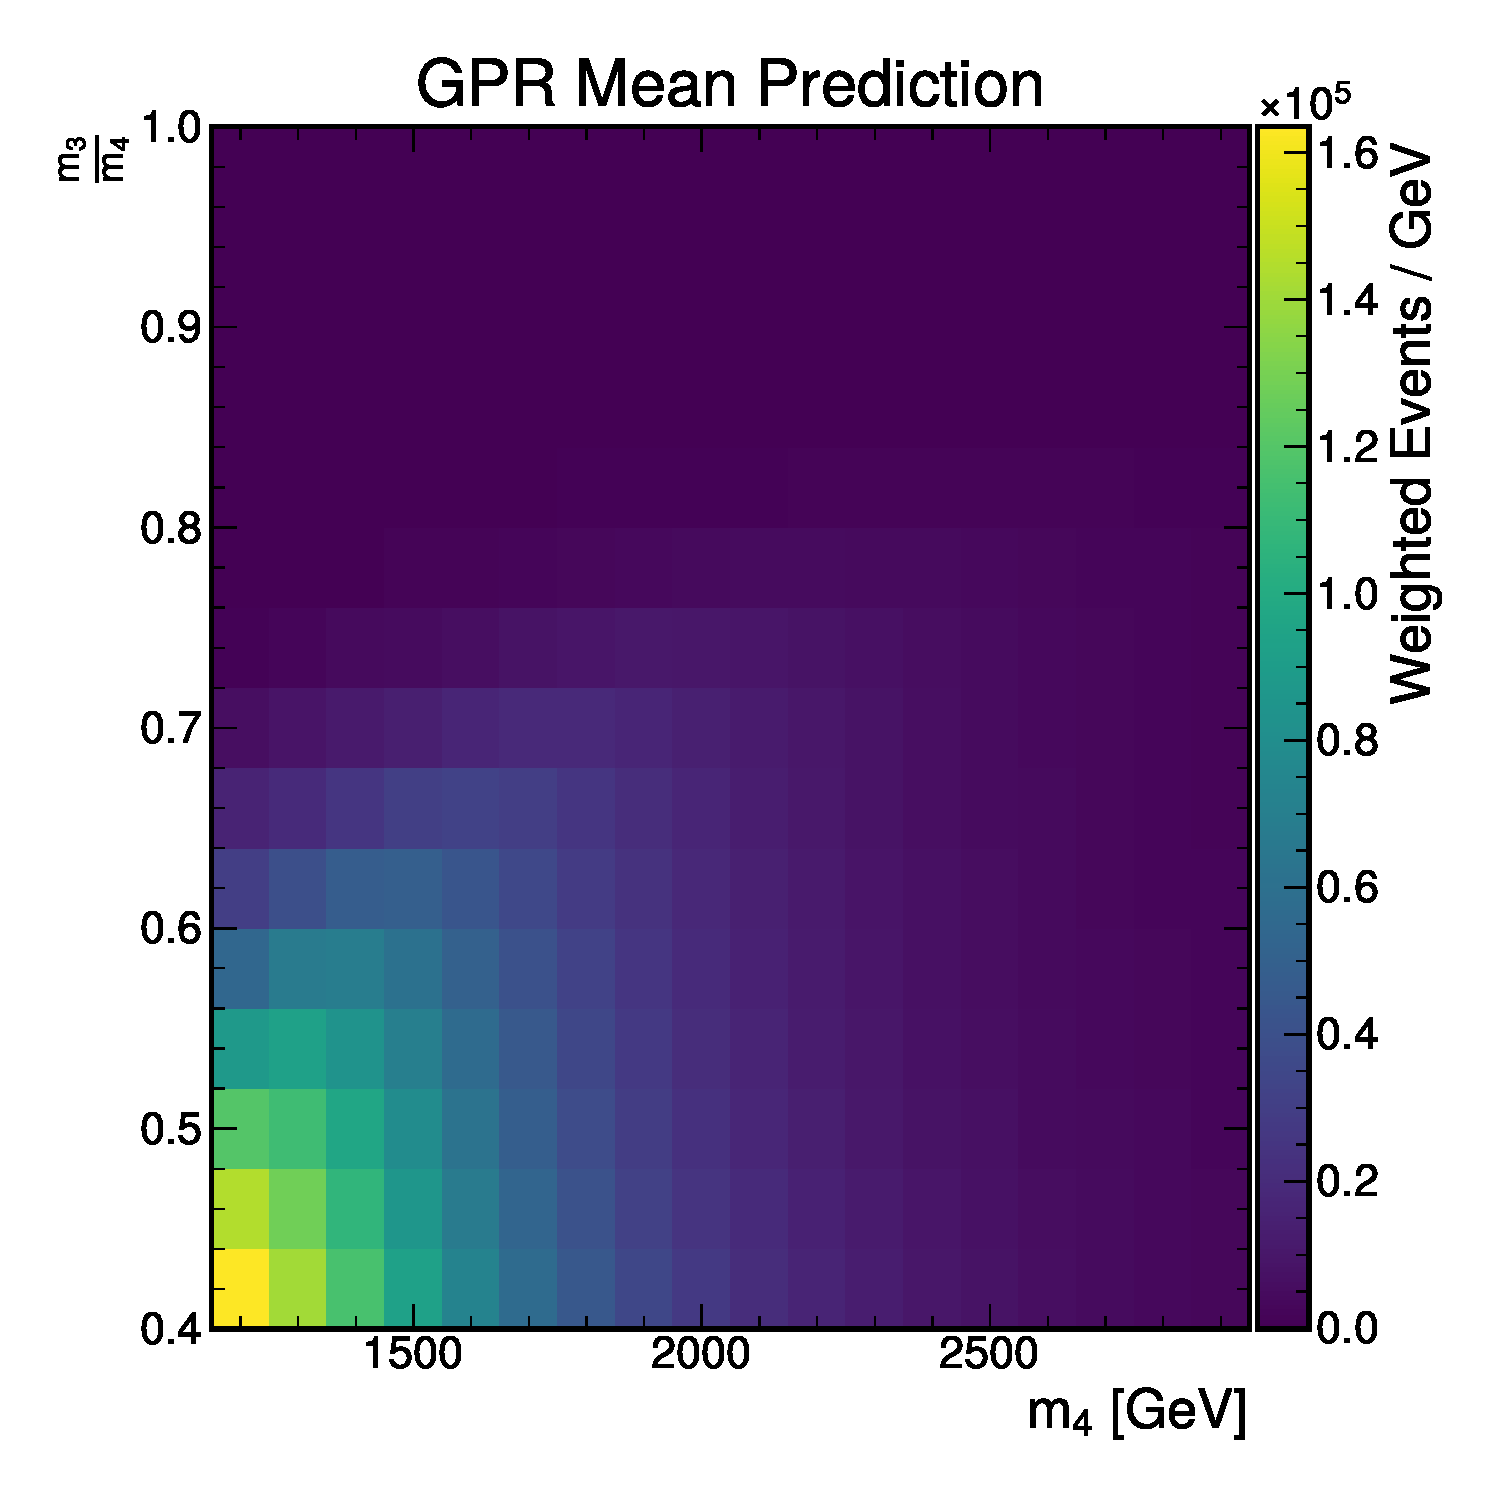
\includegraphics[width=\linewidth]{figures/#1/gpr_mean.pdf}
      \caption{}
    \end{subfigure}
    \begin{subfigure}[b]{0.45\textwidth}
      \centering
      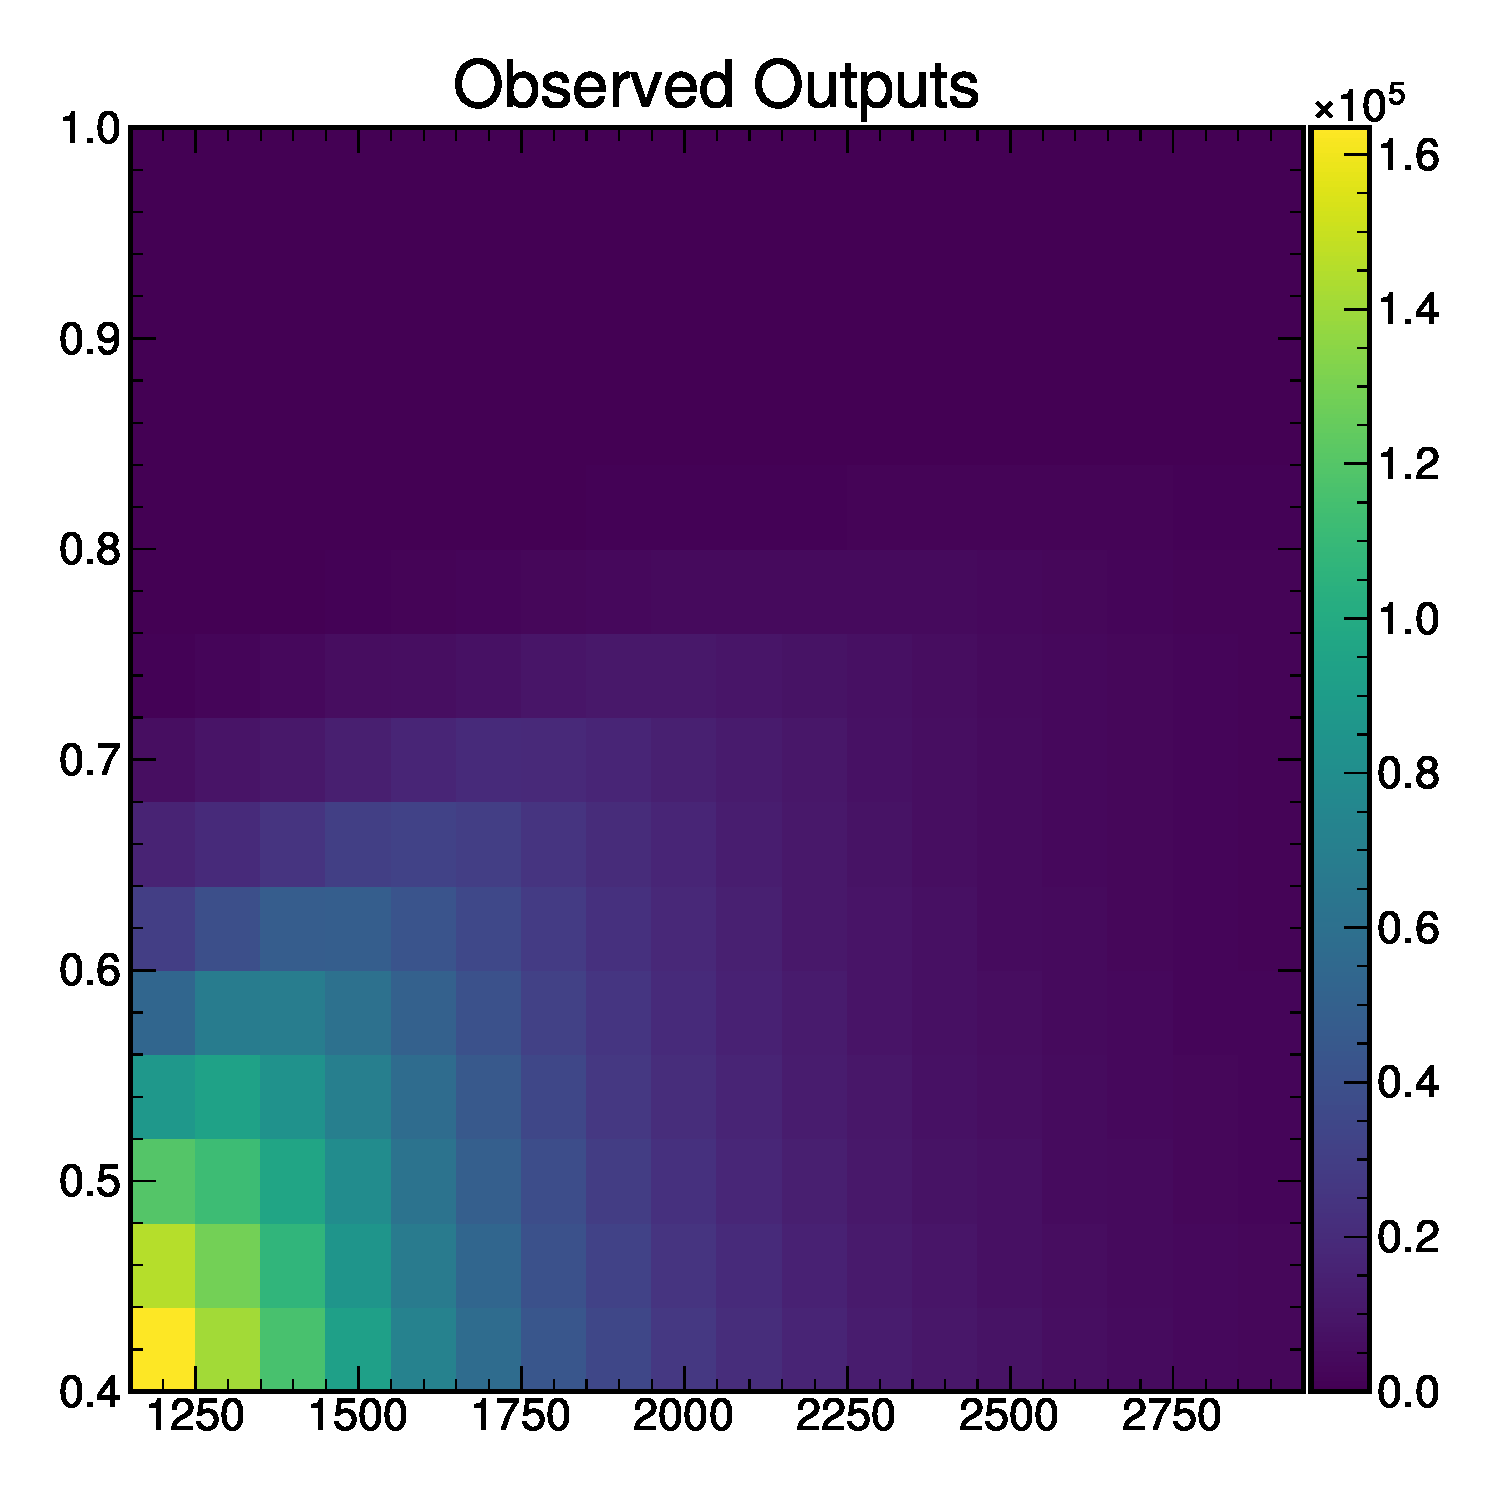
\includegraphics[width=\linewidth]{figures/#1/observed_outputs.pdf}
      \caption{}
    \end{subfigure}
    \begin{subfigure}[b]{0.45\textwidth}
      \centering
      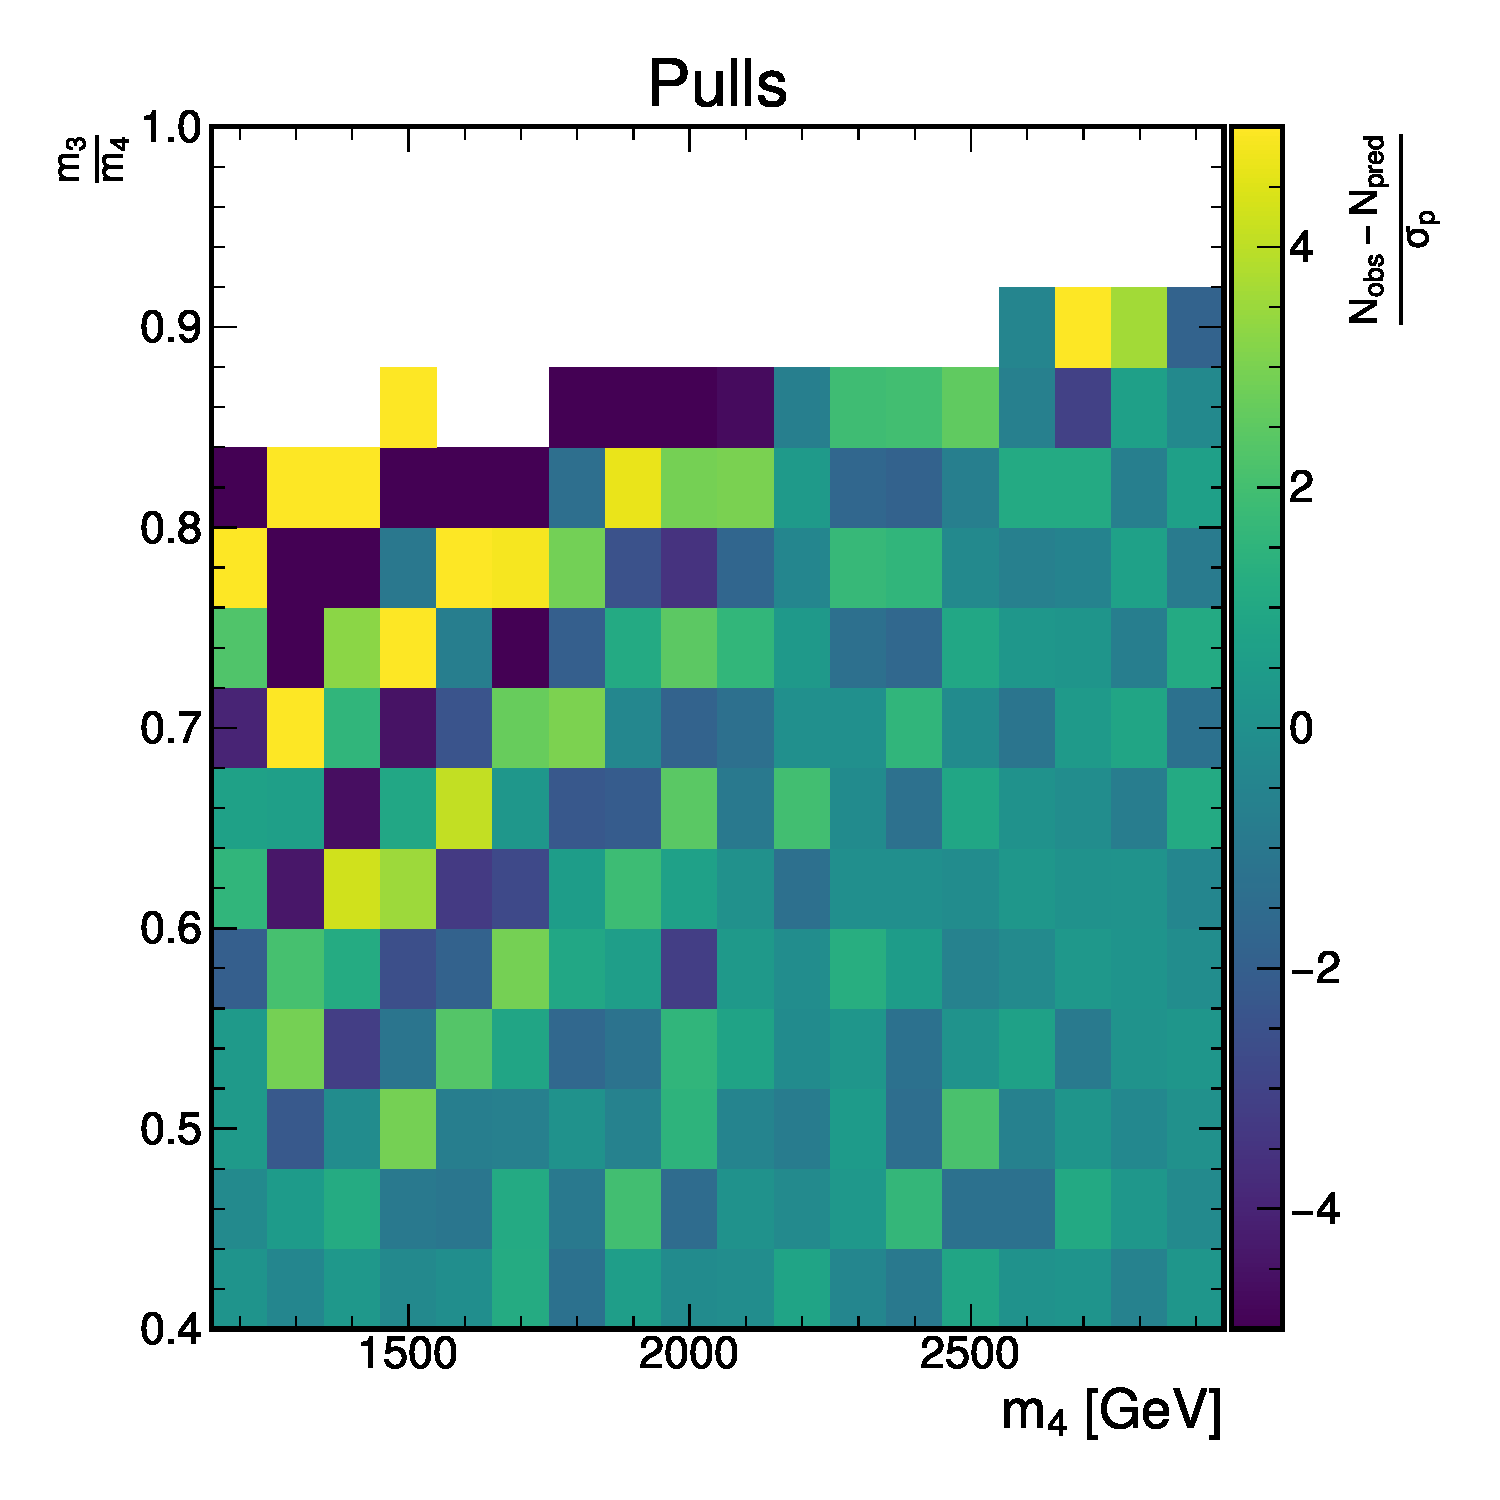
\includegraphics[width=\linewidth]{figures/#1/pulls.pdf}
      \caption{}
    \end{subfigure}
    \caption{Performing regression on control region data using the #2 kernel with #3.
      Figure (a) shows the training data
      Figure (b) shows the posterior mean found using GP regression.
      Figure (c) shows the true outputs on the entire domain.
      Figure (d) shows the pulls for each bin.}
  \end{figure}
}

\subsection{Unblinded Studies}
Of course, our estimation should perform well in the case that all points are available for training. 
\makegrid{pure_rbf}{plain RBF}{no blinding}
\makegrid{matern}{Matern}{no blinding}
\makegrid{matrix_rbf}{Matrix RBF}{no blinding}

\subsection{Blinded Studies}

\makegrid{pure_rbf_window_1300_1500__0p55_0p65}{plain RBF}{blinding around a signal of 1500,400}
\makegrid{matrix_rbf_window_1300_1500__0p55_0p65}{Matrix RBF}{blinding around a signal of 1500,400}



\end{document}


